\documentclass{article}
\usepackage{graphicx}
\graphicspath{ {./img/} }
\usepackage{amsmath}
\usepackage{amsfonts}
\usepackage{amssymb}
\usepackage{mathtools}
\usepackage[dvipsnames]{xcolor}
\usepackage{tkz-euclide} 
\usepackage[left=1.5cm, right=1.5cm, top=1.5cm, bottom=1.5cm]{geometry}

\usepackage{hyperref}
\hypersetup{
    colorlinks,
    citecolor=black,
    filecolor=black,
    linkcolor=black,
    urlcolor=black
}

\DeclareMathOperator{\Span}{span}
\renewcommand\fbox{\fcolorbox{red}{white}}
\newcommand{\sa}{\Span(\mathbb{A})}
\newcommand{\V}{\mathbb{V} (\mathbb{K})}
\newcommand{\s}[2]{#1_1, #1_2, \ldots, #1_{#2}}
\newcommand{\Vx}[1]{\mathbb{V}_#1 (\mathbb{K})}
\newcommand{\ah}{\alpha}
\newcommand{\bh}{\beta}
\newcommand{\ch}{\gamma}


\title{Algebra Lineare e Geometria Analitica}
\author{Andrea Bellu}
\date{2023/2024}

\begin{document}

\maketitle

\tableofcontents

\section{Spazi Vettoriali}
Siano $K$ un campo e $V$ un insieme. Si dice che $V$ è uno spazio vettoriale
sul campo $K$, se sono definite due operazioni: un’operazione interna binaria
su $V$, detta somma, $+: V \times V \mathbb{R}\rightarrow V$ e un’operazione
esterna, detta prodotto esterno o prodotto per scalari, $\bullet : K \times V
    \mathbb{R}\rightarrow V$, tali che:

\begin{enumerate}
    \item $(V, +)$ sia un gruppo abeliano;
    \item il prodotto esterno $\bullet$ soddisfi le seguenti proprietà:
          \begin{enumerate}
              \item $(h\cdot k)\bullet \bar{v} = h\bullet(h\bullet \bar{v}) \ \ \ \forall h,k \in K \ \ \ \text{e} \ \ \ \forall \bar{v} \in V$
              \item $(h+ k)\bullet \bar{v} = h\bullet \bar{v}+k\bullet \bar{v} \ \ \ \forall h,k \in K \ \ \ \text{e} \ \ \ \forall \bar{v} \in V$
              \item $h\bullet(\bar{v}+\bar{w}) = h\bullet\bar{v}+h\bullet\bar{w} \ \ \ \forall h,k \in K \ \ \ \text{e} \ \ \ \forall \bar{v} \in V$
              \item $1\bullet \bar{v} = \bar{v} \ \ \ \forall \bar{v} \in V$ ove 1 è l’unità del campo $K$
          \end{enumerate}
\end{enumerate}

$V(K) = (V, K, +:V\times V\mathbb{R}\rightarrow V, \bullet:K\times V\mathbb{R}\rightarrow V) \implies$ struttura algebrica

Gli elementi dell’insieme $V$ sono detti \textbf{vettori} gli elementi del
campo $K$ sono detti \textbf{scalari}.

\subsubsection{Nota bene}
Sia $\mathbb K$ un campo, indichiamo con $\mathbb K_{[x]}=\{a_0+a_1x+\cdots \ |
    \ a_i\in\mathbb K\}$ l'insieme di tutti i polinomi in $x$ a coefficienti in
$\mathbb K$.

\subsection{Vettori}
I vettori sono segmenti orientati con \textbf{verso, direzione e lunghezza}.
\begin{figure}[ht]
    \centering
    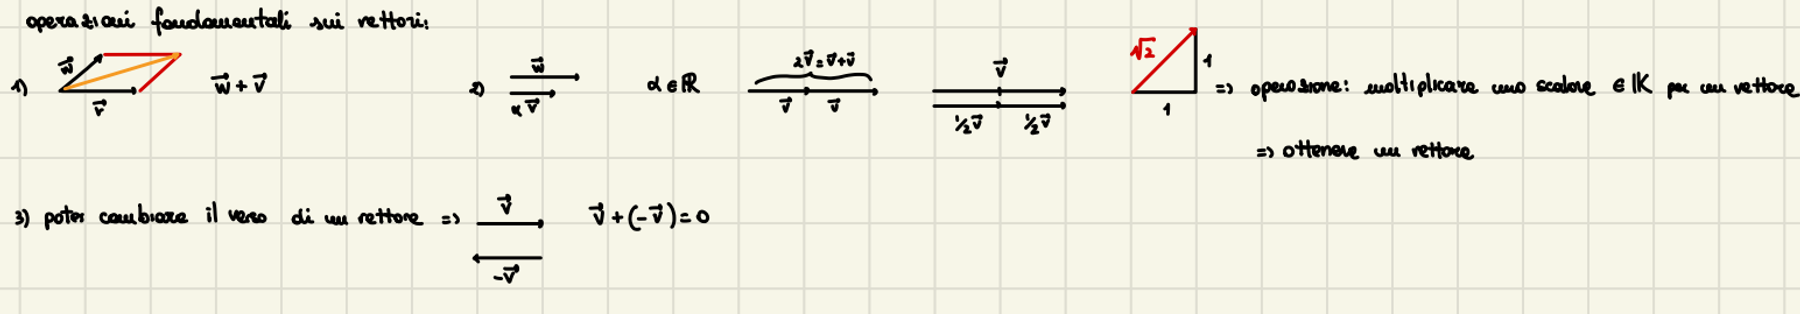
\includegraphics[width=1\linewidth]{image.png}
    \caption{Vettori}\label{fig:enter-label}
\end{figure}

\subsubsection{Esercizio}
Sia $\mathbb{R}^2$ con le operazioni di somma componente per componente
$\implies$ $(a, b) + (c, d) = (a+c, b+d)$ e prodotto per scalare campo per
campo $\alpha(a,b) = (\alpha a, \alpha b)$ è uno spazio vettoriale reale.

\begin{enumerate}
    \item Far vedere che $(\mathbb{R}^2,+)$ è un gruppo abeliano:
          \begin{enumerate}
              \item $\forall a,b \in \mathbb{R}^2 : (a,b)+(0,0) = (a+0, b+0) = (a,b) = (0+a, 0+b) = (0,0)+(a,b)$
              \item $\forall a,b \in \mathbb{R}^2 \ \ \exists \ (-a, -b) \in \mathbb{R}^2:(a,b)+(-a, -b) = (a-a, b-b) = (0,0) = (-a+a, -b+b) = (-a, -b)+(a,b)$
              \item  $\forall(a,b),(c,d),(e,f) \in \mathbb{R}^2 : (a,b)+ ((c,d)+(e,f)) = (a,b) + (c+e, d+f) = (a+ (c+e), b+ (d+f)) = ((a+c)+e, (b+d)+f) = (a+c, b+d)+(e,f)=((a,b)+(c,d))+(e,f)$
              \item  $(a,b)+(c,d)=(a+c, b+d)=(c+a,d+b)=(c,d)+(a,b)$
          \end{enumerate}
\end{enumerate}

Abbiamo verificato che $(\mathbb{R}^2,+)$ è un gruppo abeliano.

NB\@: abbiamo usato solamente che $\mathbb{R}$ è un campo $\implies$ abbiamo
usato solo le proprietà della somma
\begin{enumerate}
    \item Ora dobbiamo verificare che il prodotto esterno soddisfi le proprietà dello
          spazio vettoriale:
          \begin{enumerate}
              \item $\forall a,b,c \in \mathbb{R}^2 : 1\cdot(a,b)=(1\cdot a, 1\cdot b) = (a,b)$ $\implies$ elemento neutro
              \item $\alpha,\beta \in \mathbb{R}^2 = (\alpha\beta)\cdot(a,b)=((\alpha\beta)a, (\alpha\beta)b) = (\alpha(\beta a, \alpha(\beta b)) = \alpha(\beta a, \beta b) = \alpha(\beta \cdot(a,b))$ $\implies$ pseudo associativa
              \item $\forall \alpha,\beta\in\mathbb{R} \ \ \ (a,b) \in \mathbb{R}^2 : (\alpha+\beta)(a,b) = ((\alpha+\beta)a, (\alpha+\beta)b)=(\alpha a+\beta a, \alpha b + \beta b) = (\alpha a, \alpha b)+(\beta a, \beta b) = \alpha(a,b) + \beta(a,b)$ $\implies$ pseudo distributiva
              \item $\forall \alpha \in \mathbb{R} (a,b) ,(c,d) \in \mathbb{R}^2 : \alpha((a,b)+(c,d)) = \alpha(a+c,b+d)=(\alpha a, \alpha c, \alpha b, \alpha d)=(\alpha a, \alpha b) + (\alpha c, \alpha d) = \alpha(a,b)+\alpha(c,d)$
          \end{enumerate}

\end{enumerate}

\subsection{Combinazione Lineare}
Siano $\bar{v_1}\dots.\bar{v_k}\in V(\mathbb{K})$ vettori, $\alpha_1, \alpha_n$
scalari, si dice combinazione lineare di $(\bar{v_1}\dots\bar{v_k})$ con
$\alpha_1,\alpha_k$ il vettore $\alpha_1\bar{v_1}+\cdots+\alpha_n\bar{v_k}$.

\subsection{Applicazione Lineare}
Siano $V(\mathbb{K}) \ \ \text{e}\ \ W(\mathbb{K})$ due spazi vettoriali su
$\mathbb{K}$. Si dice applicazione lineare da $V(\mathbb{K}) \ \ \text{in} \ \
    W(\mathbb{K})$ una funzione $f:V\rightarrow W$ tale che

\[
    \forall \bar{v}, \bar{w}\in W, \forall\alpha,\beta\in\mathbb{K} \ \ \ f(\alpha\bar{w}+\beta\bar{v})=\alpha f(\bar{w})+\beta f(\bar{v})
\]
Un’applicazione lineare è una funzione che manda combinazioni lineari di
vettori in combinazioni lineari con i medesimi coefficienti. Se $V(\mathbb{K})$
è spazio vettoriale e $f:V\rightarrow W$ è applicazione lineare $\implies f(V)$
immagine di $V$ mediante $f$ è uno spazio vettoriale.

\subsection{Sottospazio Vettoriale}
Sia $W(\mathbb{K})$ uno spazio vettoriale, sia anche $X\subseteq W$
sottoinsieme $x \ne 0$, allora $X$ è detto \textbf{sottospazio} di $W$ se $X$
rispetta le operazioni di somma di vettori ristretta ad $X\times X$ e troncata
ad $X$ e di prodotto per scalari di $W$ ristretta a $\mathbb{K}\times X$ e
troncata ad $X$ soddisfa gli assiomi di spazio vettoriale. \\ In tale caso
scriviamo $X \leqslant W$. $X$ è sottospazio vettoriale se:
\begin{enumerate}
    \item la somma di due qualsiasi vettori di $X$ è un vettori di $X$
    \item il prodotto di un qualsiasi vettore di $X$ per uno scalare è ancora un vettore
          di $X$
\end{enumerate}

\subsubsection{Teorema 1}
Sia $\mathbb{V}(\mathbf{K})$ uno spazio vettoriale su $\mathbb{K}$, allora:
\begin{enumerate}
    \item $\forall\bar{v}\in V, \forall\alpha \in\mathbb{K} \ \ \alpha\cdot\bar{v} =  \underline{0} \iff \alpha = 0 \ \lor \ \bar{v}= \underline{0}$
    \item $\forall\bar{v}\in V = (-1)\bar{v} = -\bar{v}$
\end{enumerate}
\textbf{Dimostrazione}:
\begin{enumerate}
    \item Consideriamo $0 \cdot \bar{v} = (0 + 0) \cdot \bar{v} = 0 \cdot \bar{v} + 0$
          sommando a destra e a sinistra $-(0\cdot\bar v)$ si ottiene $-(0\cdot
              \bar{v})+(0\cdot \bar v) = -(0\cdot\bar v)+0\cdot\bar v+0\cdot\bar v \implies 0
              + 0 + 0\cdot\bar v \implies 0\cdot\bar v= \underline{0}$ $\alpha = 0 \implies
              \alpha\bar v = \underline{0}$. \\ Supponiamo $\alpha\bar v = \underline{0}$ con
          $\alpha = 0 \implies \exists\alpha^{-1}\in\mathbb{K} \ e \
              \alpha^{-1}(\alpha\bar v) = \alpha^-1\cdot \underline{0}$ \\
          $\alpha^{-1}(\alpha\bar v) = 1\cdot\bar v = \bar v$ \\ $\alpha^-1\cdot
              \underline{0} = \alpha^{-1}( \underline{0}+ \underline{0}) = \alpha^{-1}\cdot
              \underline{0}+\alpha^{-1}\cdot \underline{0} = \underline{0}$ $\alpha^-1\cdot
              \underline{0}=\alpha^{-1}\cdot \underline{0}+\alpha^{-1}\cdot \underline{0}$
          sommando come prima $-(\alpha^{-1}\underline 0)$ a dx e sx
          $\alpha^{-1}\underline 0 = \underline 0 \implies$ in particolare $\bar v =
              \underline 0$

    \item $(-1)\bar v + \bar v = (-1)\bar v + 1\bar v = (-1+1)\bar v = 0\cdot\underline 0 = \underline 0$ pertanto sommando a dx e sx $(-\bar v)$ otteniamo $-1\bar v = -1\bar v+\bar v+(-\bar v = \underline 0 + (-\bar v) = \underline 0 + (-\bar v)=-\bar v$
\end{enumerate}

\subsubsection{Teorema 2}
$X \leq V(\mathbb{K}) \iff X \subseteq V(\mathbb{K}) \ \text{ed} \ X$ è chiuso rispetto le combinazioni lineari di suoi elementi mediante le equazioni di $V$.
In altre parole:

\[
    \star) \ \ \forall \bar v, \bar w \in X \ \forall \alpha \beta\in\mathbb{K} : \alpha\bar v+\beta\bar w \in X
\]
\textbf{Osservazione}: $\star$ è equivalente a dire:

\[
    \bullet) \ \forall\alpha\in\mathbb K \ \ \forall \bar v\in X:\alpha\bar v+\beta\bar w \in X \ \& \ \forall\bar v,\bar w \in X: \bar v + \bar w \in X
\]
Verifichiamo che se vale $\star$ allora $\forall \alpha\in\mathbb K,
    \forall\bar v ,\bar w \in X : \alpha\bar v + \underline 0 = \alpha\bar v\in X$
e $\forall \bar v,\bar w \in X: 1\cdot\bar v + 1\cdot\bar w \in X$. \\
Viceversa se vale $\bullet$ $\implies \forall\alpha,\beta\in\mathbb K,
    \forall\bar v,\bar w \in X : \alpha\bar v,\beta\bar w \in X \implies \bar v' =
    \alpha\bar v,\bar w = \beta \bar w \in X \ \ \ \ \bar v'+\bar w' \in X \implies
    \alpha\bar v+\beta\bar w \in X$ Se vale $\bullet$ o $\star$ (stessa cosa)
allora $X$ è sottospazio. Osserviamo che molte delle proprietà di spazio
vettoriale valgono automaticamente per le restrizioni applicate a qualsiasi
$X\subseteq V(\mathbb K)$:
\begin{enumerate}
    \item se $\forall\bar v\in V: 1 \cdot \bar v = \bar v \implies \forall\bar v \in
              X:1\cdot\bar v= \bar v$
    \item $\forall\alpha,\beta \in \mathbb K \ \forall \bar v\in V:(\alpha\beta)\bar v = \alpha(\beta\bar v)\implies$vale anche per $\forall\bar v \in X$
    \item $\forall \alpha,\beta\in \mathbb K \ \forall\bar v \in V:(\alpha+\beta)\bar v=\alpha\bar v + \beta\bar v$
    \item $\forall\bar v,\bar w \ \forall \alpha\in\mathbb K=\alpha(\bar v + \bar w)=\alpha\bar v+\alpha\bar w$
\end{enumerate}
1, 2, 3, 4 valgono tutte anche sulla restrizione.
Vale anche sulle restrizioni che $\forall\bar u\bar v\bar w\in V:\bar u+(\bar v+ \bar w) = (\bar u+\bar v)+\bar w \implies \\ \implies \forall\bar u,\bar v,\bar w \in X: \bar u+(\bar v+\bar w)=(\bar u+\bar v)+\bar w$ e similmente:
$\forall\bar u,\bar v \in V: \bar u+\bar v=\bar v+\bar w \implies \forall \bar u,\bar v\in X:\bar u+\bar v=\bar v+\bar w$
\textbf{Cosa potrebbe non funzionare?}
\begin{enumerate}
    \item $\underline 0 \in X$
    \item $\forall \bar u,\bar v \in X:\bar u +\bar v\in X$
    \item $(-\bar u)\in X \ \text{se} \ \bar u \in X$
    \item $\alpha\bar u \in X \ \text{se} \ \bar u \in X \ \ \ \forall \alpha\in\mathbb K$
\end{enumerate}
Se valgono a, b, c, d possiamo troncare le operazioni ad $X \implies$ abbiamo un sottospazio.\\
b+d $\implies$ significa che si può troncare. \\
a+b+c $\implies$ $(X, +)$ un gruppo. \\

\subsection{Condizioni per sottospazio}

Se vale la condizione $\star$: $\forall\alpha,\beta\in\mathbb K \
    \forall\bar{u},\bar v\in X:\alpha\bar u+\beta\bar v\in X$
\begin{enumerate}
    \item $0\cdot\bar u + 0\cdot\bar v = \underline 0 + \underline 0 = \underline 0\in X$
    \item $1\cdot\bar u+1\cdot\bar v = \bar u+\bar v \in X$
    \item $(-1)\bar u + 0 \cdot\bar v = -\bar u +\underline 0 = -\bar u \in X \ \ \forall\bar u\in X$
    \item $\alpha\bar u+0\cdot\bar v=\alpha\bar u+\underline 0 = \alpha\bar u\in X \ \forall\bar u \in X$
\end{enumerate}
$X$ è un sottospazio, viceversa se $X$ sottospazio allora ogni combinazione lineare di suoi vettori deve stare in $X$ $\implies$ vale $\star$.

\subsection{Indipendenza e dipendenza lineare}
Siano $v_1, v_2\cdots v_n$ vettori di uno spazio vettoriale e $a_1, a_2\cdots
    a_n$ elementi del campo $\mathbb{K}$. Si dice \textbf{combinazione lineare} dei
vettori $v_1, v_2 \cdots v_n$ con coefficienti $a_1, a_2\cdots a_n$ il vettore
di $\mathbb V$.

\[a_1v_1+a_2v_2+\cdots+a_n v_n\]

\subsubsection{Sistema Libero o Legato}
$\mathbb V(\mathbb K)$ spazio vettoriale e un sistema $\mathbb A=[v_1, v_2,\ldots,v_n]$ si dice \textbf{libero}, ovvero i suoi vettori sono \textbf{linearmente indipendenti}, se l'unica combinazione lineare che dà come risultato il vettore nullo è quella con i coefficienti tutti nulli. Viceversa il sistema è \textbf{legato} e i suoi vettori sono \textbf{linearmente dipendenti}.

\subsection{Sistema di generatori di uno spazio vettoriale}
Sia $\mathbb V(\mathbb K)$ uno spazio vettoriale e sia $\mathbb A$ un sistema o
un insieme non vuoto di vettori di $\mathbb V$. Si dice \textbf{copertura
    lineare} di $\mathbb A$, e si indica $\Span(\mathbb A)$, l'insieme dei vettori
di $\mathbb V(\mathbb K)$ che si possono esprimere come combinazioni lineari,
di un numero finito, di vettori di $\mathbb A$ (tutte le possibili combinazioni
lineari).
\[
    \Span(A) = \{v\in\mathbb V \ | \ v = a_1v_1+a_2v_2+\cdots+a_n v_n,a_i v_n,a_1\in\mathbb K,v_i\in\mathbb A\}
\]

\subsubsection{Copertura Lineare = Sottospazio}
La copertura lineare $\Span(A)$ di un sistema o di un insieme $\mathbb A$, non
vuoto, di vettori $\mathbb V(\mathbb K)$ è un sottospazio vettoriale di
$\mathbb V(\mathbb K)$.\\ \textbf{Dimostrazione:} si osserva che la somma di un
numero finito di vettori di $\mathbb A$ è sempre una combinazione lineare di un
numero finito di vettori a $\mathbb A$ e, analogamente, il prodotto di un
elemento del campo $\mathbb K$, per una combinazione lineare di vettori di
$\mathbb A$, è ancora una combinazione lineare di un numero finito di vettori
di $\mathbb A$. Quindi, $\Span(A)$ è un sottospazio vettoriale di $\V$.
Pertanto, dire che $\Span(A)$ è un sottospazio vettoriale di $\V$, la copertura
lineare di un insieme o di un sistema $\mathbb A$ di vettori si suole chiamare
\textbf{spazio generato} da $\mathbb A$.\\ \textbf{Osservazione}: Diremo,
talvolta, che la copertura lineare $\sa$ di un sistema o di un insieme $\mathbb
    A$, non vuoto, di vettori di $\V$ è \textbf{il più piccolo sottospazio
    vettoriale} che contiene $\mathbb A$, nel senso che $\sa$ è contenuto in ogni
sottospazio vettoriale che contenga $\mathbb A$. E' immediato, infatti
osservare che, ogni sottospazio vettoriale che contiene $\mathbb A$ deve
contentere tutte le possibili combinazioni lineari di un numero finito di
vettori di $\mathbb A$ e, quindi, anche $\sa$.\\ Si può facilmente dimostrare
che:
\begin{enumerate}
    \item $\Span(\sa) = \sa$
    \item $\sa = \mathbb A \iff \mathbb A$ è un sottospazio vettoriale.
\end{enumerate}

\subsection{Insieme di generatori}
Sia $\V$ uno spazio vettoriale e sia $\varnothing \ne A \subseteq \mathbb V$.
Il sottoinsieme $\mathbb A$ si dice \textbf{sistema o insieme di generatori} di
$\V$ se la sua copertura lineare $\sa = \V$, cioè se \textbf{ogni vettori di
    $\V$ si può esprimere come combinazione lineare di un numero finito di vettori
    di $\mathbb A$}. (Si dice che $X$ è un \textbf{insieme di generatori} per $\V$
se $\Span(X) = V$). Ogni spazio vettoriale ammette un insieme di generatori, ma
si distinguono due casi:
\begin{enumerate}
    \item \textbf{finitamente generato:} se $\exists$ un almeno un sistema di generatori con un numero finito di vettori;
          \[
              \exists X \subseteq \V \ \ \ |X|=n \ : \ \Span(X) = V
          \]
    \item \textbf{non finitamente generato:} se ogni sistema di generatori ha un numero infinito di vettori.
\end{enumerate}

\subsubsection{Lemma}
Se $S = [\s{v}{m}]$ è un sistema di generatori di uno spazio vettoriale $\V$ e
uno dei suoi vettori $v_i$, dipende linearmente dagli altri, allora $S \ {v_i}$
è ancora un sistema di generatori di $\V$.

\subsubsection{Teorema}
Ogni spazio vettoriale $\V$ finitamente generato non banale ammette almeno un
sistema libero di generatori.

\subsection{Lemma di Steinitz}
Sia $\V$ uno spazio vettoriale f.g., sia $B=[\s{v}{n}]$ un suo sistema di
generatori e sia $A=[\s{u}{m}]$ un sistema libero di vettori di $\mathbb V$.
Allora $m\leq n$, cioè $|A|\leq|B|$.\\ \textbf{NB:} fra i vettori di $A$ e
quelli di $B$ non c'è nessuna relazione.\\ La dimostrazione non va studiata.

\subsection{Base}
Si dice \textbf{base} di uno spazio vettoriale $\V$ f.g.\ una \textbf{sequenza}
libera di generatori di $\V$. \\ Tutte la basi di uno spazio vettoriale $\V$
hanno la stessa \textit{cardinalità}.

\subsubsection{Dimostrazione}
Ci basta far vedere che ogni vettori si scrive in modo unico come combinazione
lineare degli elementi della base.\\ Supponiamo $B=(\s{b}{n})$ e $B$ sequenza
libera di generatori.\\ $\bar v \in \Span(B) \ \ \ \ \ \bar v =
    \alpha_1\bar{b_1}+\alpha_2\bar b_2 + \cdots +\alpha_n\bar b_n$.\\ Supponiamo
anche $\bar v = \beta_1\bar b_1+\beta_2\bar b_2 + \cdots +\beta_n\bar b_n$.\\
Allora $\bar{v}-\bar v = (\alpha_1\bar b_1+\cdots+\alpha_n\bar b_n) -
    (\beta_1\bar b_1+\beta_2\bar b_2 + \cdots +\beta_n\bar b_n) =
    (\alpha_1-\beta_1)\bar{b_1}+(\alpha_2-\beta_2)\bar{b_2}+\cdots+(\alpha_n-\beta_n)\bar{v_n}$.
Se $B$ libera $\implies$ deve essere $\alpha_1 = \beta_1, \alpha_2 = \beta_2
    \ldots \alpha_n = \beta_n$ perchè tutti i coefficienti sono necessariemente
$0\\ \implies B$ libera e di generatori $\iff B$ base.

\subsection{Metodo degli scarti successivi}
Algoritmo che data una sequna finita dei generatori per uno spazio vettoriale
produce $\underbar{0}$ oppure una sottosequenza libera di generatori. $S$ è di
generatori se $S= (\s{\bar{v}}{n})$ ed ogni $\bar{v}\in\V$ si scrive come
combinazione lineare di un numero finito di vettori di $S$. $V = \Span(S)$

\subsubsection{Lemma}
Sia $S=(\s{v}{n})$ una seuqenza di generatori per uno spazio vettoriale $W$
legato, allora esiste $\bar{v}_i\in S:S\smallsetminus\{\bar v_i\}$ genera $W$
(``Possiamo sempre scartare almeno un vettore da $S$ ed otteniamo ancora una
sequenza di generatori``).\\ \textbf{Dimostrazione:} $S$ legata
$\implies\exists\bar{v}_i\in S:\bar v_i=\sum_{j\ne i}^{}\ah_j\bar v_i$ \\ Sia
$\bar{w}\in\Span(S)\implies\exists\bh_j\ldots j=1\ldots n$ tali che
$\bar{w}=\bh_1\bar{v}_1+\cdots+\bh_i\bar{v}_i+\cdots+\bh_n\bar{v}_n =
    \bh_1\bar{v}_1+\cdots+\bh_i\sum_{j\ne i}^{}(\bh_j+\bh_i\ah_j)\bar{v}_j$.\\
$\implies \bar{w}$ è combinazione lineare di un numero finito di vettori di
$S\smallsetminus\{\bar{v}_i\}$\\ $\implies
    \Span(S\smallsetminus\{\bar{v}_i\})\subseteq\Span(S)$\\ Viceversa ogni vettore
di $\Span(S\smallsetminus\{\bar{v}_i\})$ è anche un vettore di
$\Span(S)\implies\Span(S\smallsetminus\{\bar{v}_i\})\subseteq\Span(S)\implies$
\fbox{$\Span(S\smallsetminus\{\bar{v}_i\})=\Span(S)$}.

\subsection{Dimensione}
Uno spazio vettoriale $\V$ ha \textbf{dimensione n}, e scriveremo $\dim\V = n$,
se $n$ è il numero di vettori che compongono una sua qualunque base.

\subsection{Componenti}
Sia $\V$ uno spazio vettoriale e $B = [\s{v}{n}]$ una sua base. $\forall v \in
    \mathbb V$ si dicono \textbf{componenti di $v$}, rispetto alla base $B$, i
coefficienti $a_1, a_2,\ldots,a_n \in \mathbb K$ tali che:
\[
    v = a_1 v_1+a_2 v_2 +\cdots+a_n v_n
\]
Cambiando l'ordine dei vettori che compaiono in una base, anche se si ottiene
ancora una bse, si tratta di una base diversa.

\subsubsection{Corollario}
In $\Vx{n}$, spazio vettoriale di dimensione n,
\begin{enumerate}
    \item $m$ vettori $\s{v}{m}$ con $m > n$ sono l.d.;
    \item $m$ vettori $\s{v}{m}$ con $m < n$ non possono generare $\Vx{n}$;
    \item una sequenza di $n$ generatori di $\Vx{n}$ risulta essere anche libera, e
          quindi, individua una base di $\Vx{n}$;
    \item una sequenza libera di $n$ vettori risulta essere anche un sistema di
          generatori e, quindi, individua una base di $\Vx{n}$.
\end{enumerate}
\textbf{Dimostrazione:}
\begin{enumerate}
    \item Dal lemma di Steinitz, se uno spazio vettoriale ha dimensione $n$, \textbf{il
              massimo numero di vettori l.d.} che si possono trovare in $\V$ è proprio $n$.
    \item Il \textbf{minimo numero di vettori che occorrono per generare} $\Vx{n}$ è
          proprio $n$.
\end{enumerate}

\subsubsection{Proposizione}
Ogni spazio vettoriale $\Vx{n}$ di dimensione $n$ contiene sottospazi di
dimensione $m \ \forall \ 0\leq m\leq n$.

\subsubsection{Proposizione}
Se $U$ e $W$ sono due sottospazi di uno spazio vettoriale $\Vx{n}$ e $U$ è
contenuto in $W$, allora:
\begin{enumerate}
    \item $\dim U\leq\dim W$;
    \item $U = W \iff \dim U = \dim W$
\end{enumerate}

\subsection{Teorema del completamento di una base}
Sia $\Vx{n}$ uno spazio vettoriale di dimensione $n$ e sia $A = (\s{v}{m})$,
ove $m\leq n$, una sequenza livera di vettori di $\Vx{n}$. Allora, in una
qualunque base $B$ di $\Vx{n}$, esiste una sequenza $B'$ di vettori, tale che
$A\cup B'$ è base di $\Vx{n}$.

\subsection{Legami fra sequenze libere, basi e matrici}
Se $B=[\s{\bar{e}}{n}]$ e $B'=[\s{\bar{e}'}{n}]$ sono due basi di $\Vx{n}$
allora:
\begin{enumerate}
    \item Esse hanno la stessa cardinalità [per Steinitz $n\leq m$ e $m\leq n \implies m
              = n$ prendendo prima $B$ come libera e $B'$ come di generatori e poi
          viceversa].\\ \textbf{Definizione:} si dice dimensione di $\Vx{n}$ il numero di
          vettori di qualunque base.
    \item Ogni vettori di $\Vx{n}$ si scrive in modo unico in componenti rispetto una
          fissata base \\ $B=(\s{\bar e}{n})\ \forall\bar v\in \Vx{n}\exists
              !(\s{\ah}{n})\in\mathbb{K}^n:\bar v = \ah_1\bar e_1+\cdots\ah_n\bar e_n$
    \item Posto $ E = \begin{bmatrix}\bar e_1 \\ \vdots \\ \bar e_n\end{bmatrix} \ e \ E'=\begin{bmatrix}\bar e'_1 \\ \vdots \\ \bar e'_n\end{bmatrix} \ \ A=\begin{bmatrix}a_{11} && a_{1n} \\ a_{n1} && a_{nn} \end{bmatrix}$ tale che $\implies E'=AE\implies$.
          \begin{enumerate}
              \item la matrice $A$ è invertibile $\implies \det(A)\ne0$
              \item se $\bar v=(\s{x}{n})E=(\s{x'}{n})E'\implies {^{t}X} = {^{t}A}{^{t}X'}$
                    cambiamento di base \\$[XE\implies\ X'E'=X'AE={^{t}X}={^{t}A}{^{t}X'}]$
          \end{enumerate}
\end{enumerate}
\textbf{Osservazione:}\begin{enumerate}
    \item Sia $S= (\s{\bar{e}}{n})$ una sequenza libera $\implies$ ogni sottosequenza di
          $S$ è libera
    \item Sia $T= (\s{g}{k})$ una sequenza di generatori $\implies$ ogni sovrasequenza di
          $T$ è di generatori.
\end{enumerate}
\begin{itemize}
    \item Se \textbf{aggiungo} vettori ad una \textbf{sequenza libera} ottengo ancora una
          sequenza libera (Teorema di completamento della base);
    \item Se \textbf{tolgo} vettori ad una \textbf{sequenza libera} ottengo ancora una
          sequenza libera;
    \item Se \textbf{aggiungo} vettori ad ua \textbf{sequenza di generatori} ottengo una
          sequenza di generatori;
    \item Se \textbf{tolgo} vettori ad una \textbf{sequenza di generatori} ottengo una
          sequenza di generatori (Metodo degli scarti successivi).
\end{itemize}

\subsubsection{Dimostrazione}
\begin{enumerate}
    \item Sia $S$ libera, supponiamo $S'\leq\ S$ legata $\implies\ S'= (\s{\bar{e}}{t})\
              \exists\ \s{\ah}{t}$ tali che
          $\ah_1\bar{e_1}+\ldots+\ah_t\bar{e_t}=\underbar{0} \\ (\s{\ah}{t}) \ne\
              (0\ldots0)
              \implies\ah\bar{e_1}+\ldots\ah_t\bar{e_t}+0\bar{e_{t+1}}+\ldots+0\bar{e_n} =
              \underbar{0}$ con $ (\s{\ah}{t}0 \ 0 \ldots0)\ne\underbar{0} \implies\ S$
          legata, \textbf{assurdo}.
    \item Sia $T= (\s{\bar{g}}{k})$ di generatori e $U= (\s{\bar{h}}{r})$ vettori
          $\implies\ T \cup\ S$ è di generatori, perchè $\forall$ vettore di $\V$ si
          scrive come $\bh_1\bar{g_1}+\ldots+\bh_k\bar{g_k} = \bh_1
              \bar{g_1}+\ldots+\bh_k \bar{g_k} + 0\bar{h_1}+\ldots+0\bar{h_r}$
\end{enumerate}

\subsection{Teorema}
Sia $\Vx{n}$ uno spazio vettoriale con $\dim(V) = n$. Sia $X\subseteq\Vx{n}$
con $|X| = n$. Allora $X = V$.

\subsubsection{Dimostrazione}
$X$ ammette una base $B'$ di n vettori $\implies$ tale base cobsta di $n$ vettori di $\Vx{n}$ liberi $\implies$ per le conseguenze di Steinitz take sequenza deve essere di generatori per $V\implies\Span(B') X\subseteq\Vx{n}=\Span(B')$ ne segue $X = V$.\\
\textbf{La nozione di dimensione ci dice ``quanto è grande'' uno spazio vettoriale.}

\subsection{Intersezione e somma di sottospazi}
Dati due sottospazi $U$ e $W$ di uno spazio vettoriale $\V$, la loro
\textbf{intersezione} e la loro \textbf{unione} sono, rispettivamente
\[
    U \cap W = \{v\in V \ | \ v\in U \text{ and } v\in W  \} \ \ e \ \ U \cup W = \{v\in V \ | \ v\in U \text{ or } v\in W  \}
\]

\subsubsection{Proposizione}
Se $U, W$ sono sottospazi di uno spazio vettoriale $\V$, $U\cap\ W$ è un
sottospazio vettoriale di $\V$.

\subsection{Somma}
Siano $U, W$ due sottospazi di uno spazio vettoriale $\V$. Si dice
\textbf{somma} $S$ di $U, W$
\[
    S = U + W = \{u+w \ | \ u \in U,w\in W\}
\]
\subsubsection{Proposizione}
La somma $S$ di due sottospazi $U, W$ di uno spazio $\V$ è uno spazio
vettoriale di $\V$.\\ \textbf{Dimostrazione:} basta osservare che se $v_1 e
    v_2$ sono vettori di $U+W$ anche $\ah{} v_1+\bh{} v_2$ appartiene a $U+W$.
Infatti se $v_1 = u_1+w_1$ e $v_2 = u_2 + w_2$ allora $\ah{} v_1 + \bh{} v_2 =
    (\ah{} u_1 + \bh{} u_2)+ (\ah{} w_1 + \bh{} w_2)$ e ciò dimostra l'asserto.

\subsection{Somma diretta}
La somma $S$ di due sottospazi $U,W$ di uno spazio vettoriale $\V$ si dice
\textbf{diretta}, e si scrive $U\oplus{W}$, se pgni vettore di $S$ si può
esprimere in modo unico, come somma di un vettore di $U$ e di uno di $W$.

\subsubsection{Proposizione}
La somma di due sottospazi $U, W$ di uno spazio vettoriale $\V$ è diretta
$\iff{U} \cap{W} = \{0\}$ \\ \textbf{Dimostrazione:} supponiamo che la somma di
$U,W$ sia diretta e sia, per assurdo, $\underbar{0} \ne{} x\in{U}\cap{} W$. Un
qualunque vettore $v$ di $U+W$ è $v=u+w$ ove $u\in{U}\text{ and } w\in{W}$, ma
anche $v= (u+x)+ (w-x)$ ove $u+x\in{U}$ e $w-x\in{W}$. Pertanto, $v$ può essere
espresso in più modi come somma di un elemento di $U$ e di uno di $W$, e questo
è assurdo.\\ Viceversa, sia $U\cap{W} = \{\underbar{0}\}$ e, per assurdo,
esista un vettore $v$ esprimibile in due modi diversi come somma di vettori di
$V$ e $W$,
\[
    v=u_1+w_1=u_2+w_2
\]
in questo caso il vettore $u_1-u_2=w_2-w_1$ sarebbe un vettore non nullo di
$U\cap{W}$ e ciò è contro l'ipotesi.

\subsubsection{Corollario}
Uno spazio vettoriale $\V$ è somma diretta di due suoi sottospazi $U, W \iff{V}
    = U+W \text{ and } U \cap{W} = \{\underbar{0}\}$

\subsection{Formula di Grassmann}
Siano $U, W$ due sottospazi di uno spazio vettoriale $\V$ f.g. Allora:
\[
    \dim(U+W) = \dim U + \dim W - \dim(U\cap W)
\]

La formula di Grassmann richiama il cosiddetto principio di
induzione/esclusione. Siano $A$ e $B$ due insiemi finiti, $\rightarrow |A \cup
    B| = |A| + |B| - |A\cap B|$.

\begin{minipage}{0.2\textwidth}
    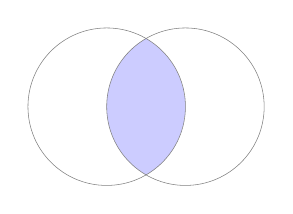
\begin{tikzpicture}
        \tkzDefPoint(0,0){A}
        \tkzDefPoint(1,0){B}
        \begin{scope}
            \tkzClipCircle(A,B) \tkzClipCircle(B,A)
            \tkzFillCircle[color=blue!20](A,B)
        \end{scope}
        \tkzDrawCircle(A,B)
        \tkzDrawCircle(B,A)
    \end{tikzpicture}
\end{minipage}%
\begin{minipage}{0.4\textwidth}
    \[
        |A\cup B| = |A\setminus B| + |A\setminus B| + |A\cap B|\]
    \[
        |A\setminus B| = |A| - |A\cap B|
    \]
    \[
        |B\setminus A| = |B| - |A\cap B|
    \]
    \[
        \implies |A\cup B| = |A\cap B| + |A| - |A\cap B| + |B| - |A\cap B| = |A| + |B| - |A\cap B|
    \]
    \vspace{2pt}
\end{minipage}

In generale se $B_u$ base di $U$ e $B_w$ base di $W$ allora $B_u\cup B_w = $
generatori di $U+W$. Ma \textbf{non è vero} che $B_u\cap B_w$ base di $U\cap
    W$. Al massimo $B_u\cap B_w$ è una sequenza libera di generatori di $U\cap W$.

\subsubsection{Conseguenza del teorema di Grassmann}
Il $max(dim (U), dim (W))\leq dim(U+W)\leq min (dim (U)+dim (W), dim (V_n))$\\
$max (0, dim (U) + dim (W) - dim(V_n))\leq dim (U\cap W)\leq min (dim (U), dim
    (W))$ \\ $U\cap W\leq U, W\leq U+W$

\subsubsection{Dimostrazione}
Idea: se $U\oplus W$ cioè $dim (U\cap W) = 0$ allora $dim (U+W) = dim (U) + dim
    (W) - 0 = dim (U) + dim (W) - dim (U\cap W)$. Supponiamo $dim (U\cap W) = i > 0
    \implies \exists$ una base $B_i$ di $U\cap W$, formata da vettori che stanno
sia in $U$ che in $W$ e sono una sequenza libera. Applicando il teorema del
completamento della base con vettori di $U$ estendiamo $B_i$ ad una base $B_u$
di $U$ (e poniamo $B_u = B_i\cup B_n'$), similmente estendiamo $B_i$ ad una
base $B_w$ di $W$ (e poniamo $B_w' = B_w \setminus B_i$).

\begin{figure}[ht]
    \centering
    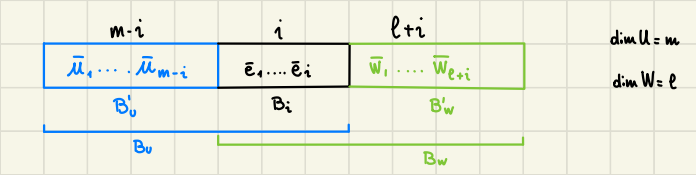
\includegraphics[width=0.7\linewidth]{grassman.png}
    \caption{Grassman}
    \label{fig:grassman}
\end{figure}

\# totale vettori = $m-i+i+l-i = m+l-i = dim U + dim U - dim U\cap W$ \\
\textbf{Osservazione:} $B_u\cup B_w = B_u'\cup B_i\cup B_w'$ è una sequenza di generatori di $U+W$ perchè unione di una base di $U$ e di una base di $W$.\\
\textbf{Dobbiamo dimostrare che è una sequenza libera:} supponiamo esistano $ (\s{\ah}{m-1}, \s{\bh}{i}, \s{\ch}{e-i})\ne\underbar{0}$ tali che
$\ah_1\bar{u}_1+\cdots\ah_{m-i}\bar{u}_{m-i}+\bh_1\bar{e}_1+\cdots+\bh_i\bar{e}_i+\cdots+\ch_1\bar{w}_1+\cdots+\ch_{l-i}\bar{w}_{l-i} = \underbar{0} \implies$ è impossibile che sia $(\s{\ah}{m-i}) = (0\ 0\cdots\ 0)$ perchè altrimenti avremmo una combinazione lineare di vettori di $B_w$ con coefficienti non tutti $0$ che dà $\underbar{0}$.
$\implies$ possiamo scrivere
\[
    \underline{\bh_1\bar{e}_1+\cdots+\bh_i\bar{e}_i+\ch_1\bar{w}_1+\cdots+\ch_{l-i}\bar{w}_{l-i}} =
\]
\[
    \substack{\in \\ \mathrm{span}(B_w) = W}
\]

\[
    \underline{= -\ah_1\bar{u}_1\cdots-\ah_{m-i}\bar{u}_{m-i}}
\]
\[
    \substack{\in \\ \mathrm{span}(B_u') \leq U}
\]
......... finire

\subsection{Definizione}
Se $U$ è un sottospazio vettoriale di $\Vx{n}$ si dice \textbf{complemento
    diretto} di $U$ in $V$, un sottospazio vettoriale $W$ di $V_n$, tale che
$U\oplus{W} = V$.

\section{Sistemi Lineari}
\subsection{Determinante}
Sia $A = (a_{ij})$ una matrice quadrata di ordine $n$, a elementi in un campo
$\mathbb{K}$. Si dice \textbf{determinante}, e si indica con $\det(A)$ o $|A|$,
la somma di tutti i suoi termini presi con il proprio segno. Cioè:
\[
    \det(A) = \sum_{\ah\in S_n}^{}sgn(\ah)a_{1\ah(1)}a_{2\ah(2)}\cdots a_{n\ah(n)}
\]

\subsubsection{Proprietà}
\begin{enumerate}
    \item Se una colonna (o una riga) di una matrice è nulla, allora il determinante è
          nullo.
    \item $\det(A) = \det({^{t}A})$, infatti, i termini estratti da ${^{t}A}$ sono tutti e soli i termini estratti da $A$. Sia $A= (a_{ij})$ e $B = ({^{t}A}) = (b_{ij})$ allora $b_{ij} = a_{ji}$. Se:
          \[
              b_{1\ah(1)}b_{2\ah(2)}\cdots b_{n\ah(n)}
          \]
          è un termine estratto da ${^{t}A}$, associato alla permutazione $\ah$, esso coincide con:
          \[
              a_{\ah(1)1}a_{\ah(2)2}\cdots a_{\ah(n)n}
          \]
          che per definizione, è un termine estratto da $A$ e individuato dalla
          permutazione $\ah^{-1}$. Dunquue, poichè $sgn (\ah) = sgn (\ah^{-1})$, possiamo
          concludere che $\det(A) = \det({^{t}A})$.
    \item Se $A'$ è ottenuta da $A$ scambiando tra loro due righe (o colonne), allora
          $\det(A') = -\det(A)$. Basta osservare che, i termini della matrice $A'$ si
          ottengono da quelli di $A$ scambiando tra loro due termini, e quindi, il segno
          del determinante cambia. Infatti, se $A'=(b_{ij})$ è ottenuta da $A= (a_{ij})$
          scambiando la k-esima riga con l'h-esima, allora ogni termine estratto da $A'$
          \[
              b_{1\ah(1)}\cdot\ldots\cdot b_{k\ah(k)}\cdot\ldots\cdot b_{h\ah(h)}\cdot\ldots\cdot b_{n\ah(n)}
          \]
          associato alla permutazione $\ah$, è uguale a:
          \[
              a_{1\ah(1)}\cdot\ldots\cdot a_{h\ah(k)}\cdot\ldots\cdot a_{k\ah(h)}\cdot\ldots\cdot a_{n\ah(n)}
          \]
          che risulta un termine di $A$ associato alla permutazione $(\sigma$ o $\ah)$,
          dove, $\sigma$ è lo scambio di $k$ con $h$. Ma essendo $sgn(\ah)=-sgn S (\ah\ o
              \ \sigma)$, risulta $|A'| = -|A|$
    \item Se $A$ ha due righe (o due colonne) uguali, allora $\det(A) = 0$. Infatti, se
          $A$ ha due righe uguali, allora, scambiando tra loro queste due righe, non si
          altera la matrice $A$, e per la precendente proprietà, $\det(A) = -\det(A)$, da
          cui $\det(A) = 0$.
    \item Se in $A$ una colonna $C_i$ è la somma di due n-uple $X_i, Y_i$, cioè se $A$ è
          del tipo:
          \[
              (C_1\ \cdots\ X_i + Y_i\ \cdots\ C_n)
          \]
          allora $|A|=|C_1 \cdots X_i \cdots C_n|+|C_1\cdots Y_i\cdots C_n|$.
          Analogamente per le righe.
    \item Se $A'$ è una matrice ottenuta da $A= (C_1 \ C_2 \cdots C_n)$ moltiplicando per
          $k\in\mathbb K$ una sua colonna (o riga), allora
          \[
              |A'|=|C_1\ \cdots\ kC_i\ \cdots\ C_n|=k|C_1\ \cdots\ C_i\ \cdots\ C_n|=k|A|
          \]
    \item Se $A$ ha due colonne (o due righe) proporzionali, allora $\det(A) = 0$.
    \item Se $A$ ha una colonna (o una riga) che è combinazione lineare di altre colonne
          (o righe), allora $\det(A) = 0$.
    \item Se $A'$ è una matrice ottenuta da $A$ sommando ad una sua colonna (o riga) un
          multiplo di un'altra colonna (o riga), allora $|A'| = |A|$.
\end{enumerate}

\subsection{Eliminazione di Gauss}
L'intendo del \textbf{metodo di eliminazione di Gauss} è quello di ridurre una
matrice $A$ ad una matrice $A'$, detta \textbf{ridotta a gradini}, in quanto il
determinante di quest'ultima può essere calcolato moltiplicando gli elementi
presenti nella diagonale principale, che ha la forma:
\[
    A' = \begin{bmatrix}
        a_{11} & a_{12} & \cdots & a_{1n} \\
        0      & a_{22} & \cdots & a_{2n} \\
        \vdots & \vdots & \ddots & \vdots \\
        0      & 0      & \cdots & a_{nn}
    \end{bmatrix}
\]
Per farlo utilizziamo quelle che si chiamano \textbf{Mosse di Gauss}:
\begin{enumerate}
    \item Scambiare tra loro due righe della matrice;
    \item Moltiplicare una riga per un numero diverso da zero;
    \item Sostituire ad una riga la somma di essa con un multiplo di un'altra riga.
\end{enumerate}
\textbf{Osservazione:} le mosse di Gauss non alterano il determinante della matrice.\\
Passi dell'algoritmo di Gauss:\\
Indichiamo con $A$ una matrice non ridotta a gradini con $m$ righe e $n$ colonne.
\begin{enumerate}
    \item Sia $C_k$, con $1\leq\ k\leq\ n$, la prima colonna a paritre da sinistra che
          contiene almeno un termine $a$ non nullo.\\ Detta $R_1$ la prima riga della
          matrice, possono presentarsi\textbf{ due eventualità}:
          \begin{enumerate}
              \item Se $a$ è un elemento di $R_1$, passiamo al punto $3$
              \item Se $a\notin\ R_1$. Controlliamo se la matrice ottenuta dopo lo scambio è
                    ridotta a gradini: se lo è possiamo fermarci, in caso contrario procediamo
                    oltre.
          \end{enumerate}
    \item L'obiettivo è annullare tutti gli elementi della k-esima colonna al di sotto di
          $a$. Sostituiamo ogni riga $R_i$, con $i>1$ e con k-esimo elemento non nullo,
          con $R_i+\lambda\ R_1, \lambda\in\mathbb{R}: \ R_i+\lambda\ R_1 = 0$.
    \item Se la matrice risultante è ridotta a gradini, allora l'algoritmo termina,
          altrimenti ripetiamo i passi precedenti con la matrice ottenuta.
\end{enumerate}

\subsection{Complemento algebrico}
Sia $A= (a_{ij})$ una matrice quadrata di ordine $n$, a elementi in un campo
$\mathbb{K}$. Si dice \textbf{complemento algebrico} dell'elemento $a_{hk}$, e
si indica con $\Gamma_{hk}$, il determinate della matrice quadrata di orfdine
$n-1$, ottenuta da $A$ cancellando la riga $h$ e la colonna $k$, preso con il
segno $ (-1)^{h+k} $.

\subsection{Teorema di Laplace I}
Data una matrice quadrata $A$ di ordine $n$, la somma dei prodotti degli
elementi di una sua riga (o colonna), per i rispettivi complementi algebrici, è
il determinate di $A$. Pertanto, la formula del calcolo del determinanto di $A=
    (a_{ij})$ rispetto alla i-esima riga è:
\[
    |A| = \sum_{j=1}^n a_{ij}\Gamma_{ij} \ \ \forall i = 1, 2, \ldots, n
\]
Rispetto alla j-esima colonna è:
\[
    |A| = \sum_{i=1}^n a_{ij}\Gamma_{ij} \ \ \forall j = 1, 2, \ldots, n
\]
L'utilizzo dei complementi algebrici consente, quindi il calcolo del
determinante di una matrice di ordine $n$ calcolando determinanti di matrici di
ordine inferiore.

\subsection{Teorema di Laplace II}
Sia $A$ una matrice quadrata di ordine $n$. La somma dei prodotti degli
elementi di una sua riga (o colonna) per i complementi elgebrici degli elementi
di un'altra riga (o colonna) vale zero.

\subsection{Teorema di Binet}
Date due matrici quadrate di ordine $n$, $A$ e $B$, il determinante della
matrice prodotto $AB$ è uguale al prodotto dei determinanti delle due matrici:
\[
    |AB| = |A||B|
\]

\subsection{Matrici Invertibili}
Una matrice quadrata $A$ di ordine $n$ si dice \textbf{invertibile} se esiste
una matrice $B$ quadrata e dello stesso ordine, tale che $AB = BA = I_n$, dove
$I_n$ è la matrice identità di ordine $n$. In tal caso, la matrice $B$ si dice
\textbf{matrice inversa} di $A$ e si indica con $A^{-1}$.

\subsubsection{Teorema}
Una matrice quadrata $A = (a-{ij})$, di ordine $n$, è invertibile
$\iff|A|\ne0$. In questo caso, la matrice inversa di $A$ risulta essere
$A^{-1}=|A|^{-1}\ {^{t}A_a}$ dove ${^{t}A_a}$ è la trasposta dell'aggiunta di
$A$.

\subsection{Dipendenza lineare e determinanti}
Data una matrice $A\in{\mathbb{K}^{m,n}} (K)$ si dice \textbf{minore di ordine
    k}, estratto da $A$, una matrice quadrata di ordine $k$ (ovviaente $k\leq{m}$ e
$k\leq{n}$) ottenuta da $A$ cancellando $m-k$ righe e $n-k$ colonne.\\

\subsubsection{Teorema}
Una sequenza $S = (\s{v}{k})$ di $k$ vettori $ (k\leq{n})$ dello spazio
vettoriale $\Vx{n}$ è libera $\iff$ dalla matrice $A$, che ha nelle proprie
righe (o colonne) le componenti dei vettori di $S$ in una base $B$ di $\Vx{n}$,
si può estrarre un minore di ordine $k$ con determinante non nullo.

\subsection{Rango}
Sia $A$ una matrice di $K^{m,n} (\mathbb{K})$. Si dice \textbf{rango} della
matrice $A$, e si indica con $rK (A)$, il massimo ordine di un minore non nullo
estratto da $A$.\\ In modo equivalente, il rango di una matrice $A$ è $p$
quando esiste un minore di ordine $p$ non nullo, ma non esiste alcun minore di
ordine $p+1$ non nullo.\\

\subsubsection{Osservazioni}
Data una matrice $A \in K^{m,n} (\mathbb{K})$
\begin{enumerate}
    \item $rK (A) = 0\iff{} A$ è la matrice nulla;
    \item il rango di $A$ coincide con il rango della sua trasposta ${^{t}A}$;
    \item $rK (A) \leq min\{m,n\}$;
    \item se $B$ è una matrice di $K^{n,p} (\mathbb{K})$, il rango della matrice prodotto
          $AB$ è minore o guale, si adel rango di $A$, che di queòòp di $B$.
    \item se $A$ e $B$ sono matrici quadrate dello stesso ordine e $A$ è invertibile,
          allora $rK (AB) = rK (BA) = rK (B)$.
\end{enumerate}

\subsection{Kronecker}
Gli spazi vettoriali $\Span(R)$ ed $\Span(C)$, di una matrice $A\in K^{m,n}
    (\mathbb{K})$, hanno la stessa dimensione e tale dimensione coincide con il
rango di $A$.

\subsection{Osservazione}
Il rango di una matrice $A$ coincide con il massimo numero di righe o di
colonne linearmente indipendenti estraibili dalla matrice $A$.

\subsubsection{Corollario}
Se $A$ è una matrice quadrata di ordine $n$, con elementi in un campo
$\mathbb{K}$, le seguenti condizioni sono equivalenti:
\begin{enumerate}
    \item $|A|\ne0$;
    \item $A$ è invertibile
    \item $rK (A) = n$;
    \item le righe sono linearmente indipendenti e, quindi sono base di $\mathbb{K}^n$;
    \item le colonne sono linearmente indipendenti e, quindi sono base di $\mathbb{K}^n$;
\end{enumerate}

\subsection{Teorema degli orlati}
Una matrice $A\in K^{m,n} (\mathbb{K})$ ha rango $r$ se e solo se esiste un
minore $M$ di ordine $r$ a determinante non nullo e tutti i minori di ordine
$r+1$, che contengono $M$, hanno determinante nullo.

\subsection{Sistemi Lineari}
Un \textbf{sistema lineare} è insieme di $m$ equazioni lineari in $n$ incognite
a coefficineti in un campo $\mathbb{K}$, un sistema lineare si può
rappresentare come:
\[
    \begin{cases}
        a_{11}x_1 + a_{12}x_2 + \cdots + a_{1n}x_n = b_1 \\
        a_{21}x_1 + a_{22}x_2 + \cdots + a_{2n}x_n = b_2 \\
        \vdots                                           \\
        a_{m1}x_1 + a_{m2}x_2 + \cdots + a_{mn}x_n = b_m
    \end{cases}
\]
con $a_{ij}, b_i \in \mathbb{K}$. Gli elementi $a_{ij}$ si chiamano
coefficienti delle incognite, gli elementi $b_i$ si chiamano termini noti.\\ La
matrice $m\times n$
\[
    A = \begin{bmatrix}
        a_{11} & a_{12} & \cdots & a_{1n} \\
        a_{21} & a_{22} & \cdots & a_{2n} \\
        \vdots & \vdots & \ddots & \vdots \\
        a_{m1} & a_{m2} & \cdots & a_{mn}
    \end{bmatrix}
\]
è detta matrice dei coefficienti o \textbf{matrice incompleta} del sistema.\\
La matrice $n\times 1$
\[
    X = \begin{bmatrix}
        x_1    \\
        x_2    \\
        \vdots \\
        x_n
    \end{bmatrix}
\]
è detta matrice delle incognite.\\
La matrice $m\times 1$
\[
    B = \begin{bmatrix}
        b_1    \\
        b_2    \\
        \vdots \\
        b_m
    \end{bmatrix}
\]
è detta matrice dei termini noti.\\
Infine, la matrice $m\times (n+1)$
\[
    A|B = \begin{bmatrix}
        a_{11} & a_{12} & \cdots & a_{1n} & b_1    \\
        a_{21} & a_{22} & \cdots & a_{2n} & b_2    \\
        \vdots & \vdots & \ddots & \vdots & \vdots \\
        a_{m1} & a_{m2} & \cdots & a_{mn} & b_m
    \end{bmatrix}
\]
è detta \textbf{matrice completa} del sistema.

\subsubsection{Sistema omogeneo}
Un sistema lineare si dice \textbf{omogeneo} se tutti i termini noti sono
nulli. Utilizzando il prodotto tra matrici, il sistema lineare assume la
seguente forma:
\[
    AX = B
\]
In particolare, un sistema lineare omogeneo, in forma matriciale, si scrive
\[
    AX = \underbar{0}
\]
Si è soliti chiamare \textbf{sistema lineare omogeneo associato} ad $AX = B$,
il sistema lineare omogeneo ottenuto da $AX = B$ ponendo $B = \underbar{0}$.

\subsubsection{Sistema compatibile}
Sia $AX = B$ un sistema lineare in $m$ equazioni e $n$ incognite. Si dice che
tale sistema ha soluzione, ovvero che il \textbf{sistema è compatibile}, se
esiste almeno un $n$-upla $ (\s{\ah}{n})$ di elementi di $\mathbb{K}$ che
risolve tutte le equazioni del sistema. Tale $n$-upla è detta
\textbf{soluzione}.\\ \textbf{Osservazione:} affermare hce una $n$-upla $
    (\s{\ah}{n})$ di elementi di $\mathbb{K}$ è soluzione di un sistema $AX = B$,
pensando tale sistema scritto nella forma, equivale a dire che
\[
    \ah_1C_1 + \ah_2C_2 + \cdots + \ah_nC_n = B
\]
cioè che $B$ è combinazione lineare delle colonne della matrice $A$ secondo i
coefficienti $\ah_1, \ah_2, \ldots, \ah_n$.

\subsection{Rouché-Capelli}
Un sistema lineare $AX = B$, in $m$ equazioni e $n$ incognite, è compatibile
$\iff rk (A) = rk (A|B)$.

\subsubsection{Dimostrazione}
Se il sistema $AX = B$ ha soluzione, esiste una $n$-upla di $\mathbb{K}$ $
    (\s{\ah}{n})$, che ne soddisfa tutte le equazioni, tale, cioè, che:
\[
    \ah_1C_1 + \ah_2C_2 + \cdots + \ah_nC_n = B
\]
e quindi, B risulta essere combinazione lineare delle colonne della matrice A.
Pertanto, il massimo numero di colonne linearmente indipendenti, estraibili
dalla matrice $A$, coincide con il massimo numero di colonne linearmente
indipendeti, estraibili dalla matrice $A|B$, e $rK (A) = rK (A|B)$. Viceversa
se $rK (A) = rK (A|B)$, allora il massimo numero di colonne linearmente
indipendenti, estraibili dalla matrice $A$, coincide con il massimo numero di
colonne linearmente indipendenti, estraibili dalla matrice $A|B$, di
conseguenza, la colonna $B$ risulta una combinazione lineare delle colonne
della matrice $A$, e quindi, esiste una $n$-upla di $\mathbb{K}$ $
    (\s{\ah}{n})$, tale che:
\[
    \ah_1C_1+\ah_2C_2+\cdots+\ah_nC_n = B
\]
Pertanto, il sistema $AX = B$ ha soluzione.

\subsection{Cramer}

\end{document}